\documentclass[twoside,11pt]{article}

% Any additional packages needed should be included after jmlr2e.
% Note that jmlr2e.sty includes epsfig, amssymb, natbib and graphicx,
% and defines many common macros, such as 'proof' and 'example'.
%
% It also sets the bibliographystyle to plainnat; for more information on
% natbib citation styles, see the natbib documentation, a copy of which
% is archived at http://www.jmlr.org/format/natbib.pdf

\usepackage{jmlr2e}

\usepackage{booktabs}
%\usepackage{graphicx}
\usepackage[tableposition=top]{caption}
\usepackage{lipsum}
\usepackage{diagbox}
\usepackage{rotating}
\usepackage{subcaption}
\usepackage{multirow}
\usepackage{wrapfig}
\usepackage{minted}
\usepackage{framed}

% Definitions of handy macros can go here

\newcommand{\dataset}{{\cal D}}
\newcommand{\fracpartial}[2]{\frac{\partial #1}{\partial  #2}}

% Heading arguments are {volume}{year}{pages}{date submitted}{date published}{paper id}{author-full-names}

% \jmlrheading{1}{2000}{1-48}{4/00}{10/00}{meila00a}{Marina Meil\u{a} and Michael I. Jordan}

% Short headings should be running head and authors last names

\ShortHeadings{Performance of Six Algorithms on Five Binary Classification Problems}{Siemers}
\firstpageno{1}

\begin{document}
	
	\title{Empirical Study of the Performance of Six Algorithms on Five Binary Classification Problems}
	
	\author{\name Maximilian Siemers \email siemersm@gmail.com \\
		\addr Department of Cognitive Science\\
		University of California, San Diego\\
		San Diego, CA 92117, USA}
	
	\course{COGS 118A: Introduction to Machine Learning I}
	\prof{Prof. Zhuowen Tu}
	
	\maketitle
	
	\begin{abstract}%   <- trailing '%' for backward compatibility of .sty file
		
	\end{abstract}
		Using five-fold cross-validation, three different train-test splits of the datasets, and three random dataset shuffles, the algorithms KNN, Logistic Regression, Decision Trees, Bagged Trees, Boosted Trees, and Random Forest were trained on five different data sets. The influence of several hyperparameters' values on prediction accuracy was visualized and, using the best hyperparameter value combination in each loop, testing accuracy was determined. Averaging over the random shuffles of the data sets, the observed overall ranking order of the classifiers was almost identical to that reported in existing literature. For almost all hyperparameters, their influence on testing accuracy seemed to follow a systematic relationship, which confirms the validity of recent approaches in machine learning to automatically learn optimal hyperparameter values.
	
	Word Count: $\approx 2300$
	
	\section{Introduction}
		In the realm of machine learning algorithms, there are two kinds of parameters to be distinguished. First, there are the parameters that the algorithm seeks to learn from the data that it is trained on. These parameters are often called weights and determine the algorithm's transformation from the data input space to the prediction outcome space. Then, on a more abstract layer, there are the hyperparameters, which determine \textit{how} the algorithm learns from the data. They often constrain the learning process, assign weight to different loss functions, or influence tweaking strategies such as pruning or regularization.
		
		In machine learning practice (specifically in UCSD COGS 118A homework assignments), hyperparameters are usually either left at their default values or determined by exhaustive grid search. This approach leaves little space for understanding the role of the hyperparameters in influencing the algorithm's quality of fit. Moreover, it might be interesting to investigate whether there exists a systematic relationship between algorithm hyperparameter values, the problem data set used, and the overall prediction accuracy of the algorithm. Getting more insight into this relationship might be helpful to make the search for optimal prediction algorithms both more efficient and automated. For an example approach of automated hyperparameter tuning by applying machine learning to machine learning, see the paper \textit{Learning to learn by gradient descent by gradient descent} from Google DeepMind \citep{andrychowicz_learning_2016}.
		
		Before this background is the motivation of the present study: to visualize and better understand how several binary classifiers' hyperparameters influence training and testing accuracy on different data sets. The goal is to use cross-validation, several different train-test-splits and multiple random samples from the datasets to achieve reliable results. In addition, the average testing accuracies of all classifiers on each of the problem data sets shall be compared to investigate whether they can replicate the results from the comprehensive empirical classification performance study by \cite{caruana_empirical_2006}.
	
	\section{Method}
		\subsection{Problems}
			Five supervised binary classification problem data sets that are available at the UCI Machine Learning database \citep{dheeru_uci_2017} were used for this analysis: The Covertype Data Set (\textit{COVTYPE}), the Census Income Data Set (\textit{INCOME}), the Letter Recognition Data Set (\textit{LETTER}), the Iris Data Set (\textit{IRIS}), and the Breast Cancer Wisconsin (Original) Data Set \citep[\textit{WDBC},][]{mangasarian_cancer_1990}. All of these five data sets consist of rows with sample observations and columns with features. The binary classification target was either included in the data set download (INCOME, IRIS, WDBC) or created from an existing multi-class target (COVTYPE, LETTER).
			
			The following paragraphs describe the purposes of each of the five data sets and give examples of their features.
			
			\paragraph{COVTYPE}
			Predictors are quantitative and qualitative measurements of cartographic variables for 30x30 meter cells from US Geological Survey (USGS) and US Forest Service (USFS) data. The outcome is a class of seven forest cover types as determined by the USFS Region 2 Resource Information System (RIS) data. The largest outcome class is interpreted as a positive outcome. \textit{Predictor examples}: \textit{Elevation} measured in meters, \textit{Soil Type} as indicated by one of 40 classes.
			
			\paragraph{INCOME}
			Predictors are quantitative and qualitative US Census data. The outcome is the yearly income of a given subject, indicated by either >\$50k/y or <\$50k/y. The first is interpreted as a positive outcome, the second as a negative. \textit{Predictor examples}: \textit{Age} in years, \textit{Relationship} as one of the class Wife, Own-Child, Husband, Not-in-family, Other-relative, Unmarried.
			
			\paragraph{LETTER}
			Predictors are quantitative numerical attributes (statistical moments and edge counts) of a large number of black-and-white rectangular pixel displays of the 26 capital letters in the English alphabet. The outcome is the English letter, where letters A-L were used as a positive and letters M-Z were used as negative outcomes. \textit{Predictor examples}: mean x y correlation, correlation of y-edges with x.
			
			\paragraph{IRIS}
			Predictors are sepal and petal width and length of iris plants. The outcome is the class of three types of iris plants. The first class (Iris Setosa) was used as a negative outcome, the second (Iris Versicolor) as a positive outcome.
			
			\paragraph{WDBC}
			Predictors are quantitative measurements of attributes of breast cancer samples. The outcome is the class of benign and malignant diagnosis results, where benign was interpreted as a negative and malignant as a positive outcome. \textit{Predictor examples}: \textit{Clump Thickness (1-10)}, \textit{Uniformity of Cell Shape} (1-10). The data stem from University of Wisconsin Hospitals.
			
			\vspace{1em}
			
			In order to reduce the running time of the analysis, which is based on heavily nested loops, to a reasonable amount, the number of observations in all datasets with $|DATASET| > 2000$ was limited to 2000 randomly drawn samples. Table \ref{tab:data_sizes} lists the resulting and original data set sizes.
			
			% tab:data_sizes - Data size table
			\begin{wraptable}{l}{.52\linewidth}
				\captionbox{Original and limited sizes of data sets\label{tab:data_sizes}}{
				\begin{tabular}{lll}
					\toprule
					\textbf{Data set} & \textbf{Orig. Size} & \textbf{Lim. Size} \\
					\midrule
					COVTYPE	& $(581011 \times 55)$	& $(2000 \times 55) $ \\
					INCOME	& $(32561 \times 109)$	& $(2000 \times 109) $ \\
					LETTER	& $(20000 \times 16)$	& ($2000 \times 16) $ \\
					IRIS	& \multicolumn{2}{c}{--- $(150 \times 5)$ ---} \\
					WDBC	& \multicolumn{2}{c}{--- $(569 \times 31)$ ---} \\
					\bottomrule
				\end{tabular}}
			\end{wraptable}
	
		\subsection{Classifier Algorithms}
			\label{sec:clf_hyperparams}
			Six classification algorithms were trained on the data sets described above: K Nearest Neighbors (\textit{knn}), Logistic Regression (\textit{logreg}), Decision Trees (\textit{dt}), Bagged Decision Trees (\textit{bagdt}), Boosted Decision Trees (\textit{bstdt}), and Random Forest (\textit{rf}). All were implemented in Python using the corresponding classes from the \textit{scikit-learn} package. The following paragraphs describe the hyperparameters that were varied in grid search and considered in analyzing their influence on classification performance.
			
			\paragraph{K Nearest Neighbors (knn)}
			$K$ was varied to assume all values between $K=1$ and $K=30$, and, if $|DATASET|>30$, in the set of 10 additional values that were evenly spread between 30 and $|DATASET|$. If $\frac{|DATASET|}{cv\_fold} < 30$, then the range of values for $K$ was limited to $\frac{|DATASET|}{cv\_fold}$.
			
			\paragraph{Logistic Regressoin (logreg)}
			The inverse regularization parameter $C$ was varied between $10^{-8}$ and $10^4$ in factors of 10. Larger values of $C$ allow the parameters of the model to vary more freely.
			
			\paragraph{Decision Tree (dt)}
			Two Decision Tree hyperparameters were varied: \textit{max\_depth} determines the maximum depth that a tree is allowed to grow and was varied to assume values between 1 and 29. \textit{max\_features} determines how many features are considered when finding the best split and was also varied between 1 and 29 (or $n_{features}$ in the data set if $n_{features} < 29$) in steps of 1.
			
			\paragraph{Bagged Decision Trees (bagdt)}
			The number of Decision Tree estimators in the ensemble \textit{n\_estimators} was varied to assume values between 1 and 29 in steps of 1.
			
			\paragraph{Boosted Decision Trees (bstdt)}
			Same manipulations as in Bagged Decision Trees.
			
			\paragraph{Random Forest (rf)}
			\textit{max\_features} determines how many features are considered when finding the best split at each tree in the forest and was varied to assume all values in $\{1, 2, 4, 6, 8, 12, 16, 20\}$ that were smaller or equal to $n_{features}$. The number of trees in the forest \textit{n\_estimators} was set to 1024.
			
			
	
	\section{Experiments}
		
		Each of the five data sets (see Table \ref{tab:data_sizes}) was divided into training and testing sets for each of the relative training sizes .5, .2, and .8 (\textit{train splits}). In order to exclude the random sampling procedure as a potential confounding cause of results, the splits into training and testing sets were repeated three times each (\textit{shuffles}) with varying random seeds, thus resulting in nine analysis loops.
		
		Within each loop, an exhaustive grid search for all combinations of hyperparameters (see Section \ref{sec:clf_hyperparams}) of all classifiers was run on each problem data set. The parameter search was conducted using five-fold cross-validation. The averaged cross-validated prediction accuracies for each algorithm, data set, train split run, and random shuffling run were saved for later analysis.
		
		\subsection{Prediction Accuracy by Hyperparameter}
			Figures \ref{fig:hyperparam_knn_dt} and \ref{fig:hyperparam_others} depict the relationships between hyperparameter values and cross-validated prediction accuracy score. The performance metrics are averaged across problems, shuffles, and train splits. For Decision Trees, where two different hyperparameters were varied, each of their corresponding plots shows performance averaged over the varying values of the other hyperparameter.
			
			% Hyperparam figures # 1
			\begin{figure}[h]
				\begin{framed}
					\centering
					
					\begin{subfigure}[b]{.49\linewidth}
						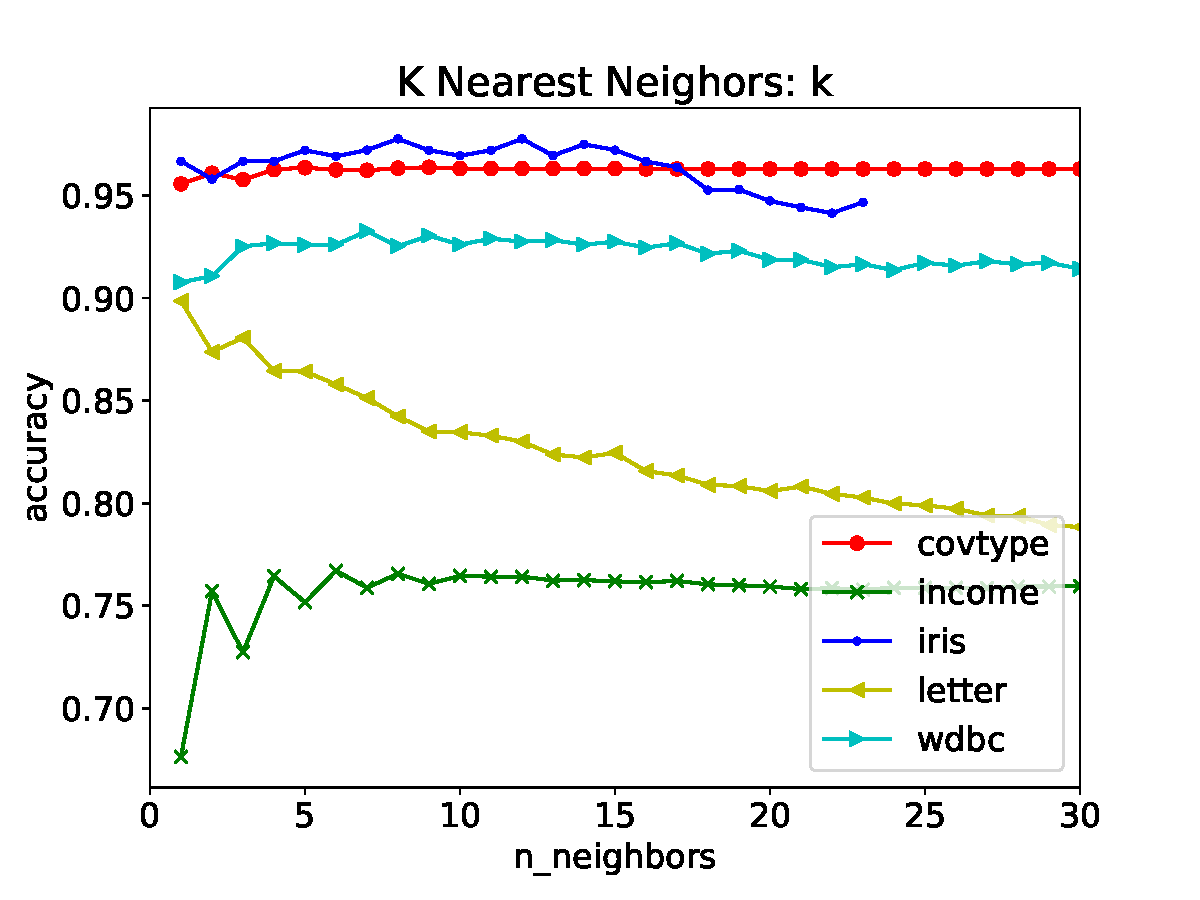
\includegraphics[width=\linewidth]{knn_hyperparam_zoomed}
						\caption{KNN: \textit{k}}
						\label{fig:hyperparam_knn_zoomed}
					\end{subfigure}
					\begin{subfigure}[b]{.49\linewidth}
						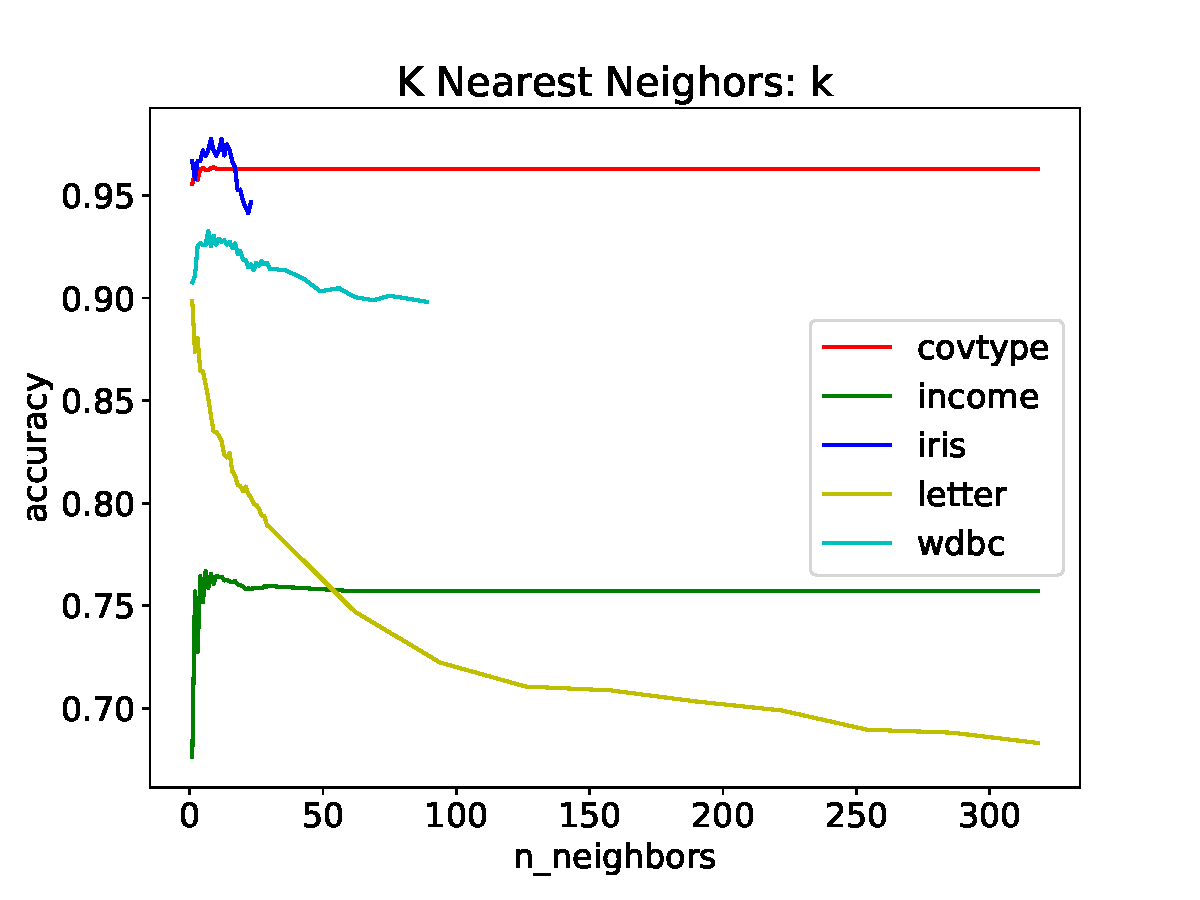
\includegraphics[width=\linewidth]{knn_hyperparam_all}
						\caption{KNN: \textit{k}}
						\label{fig:hyperparam_knn_all}
					\end{subfigure}
				
					\begin{subfigure}[b]{.49\linewidth}
						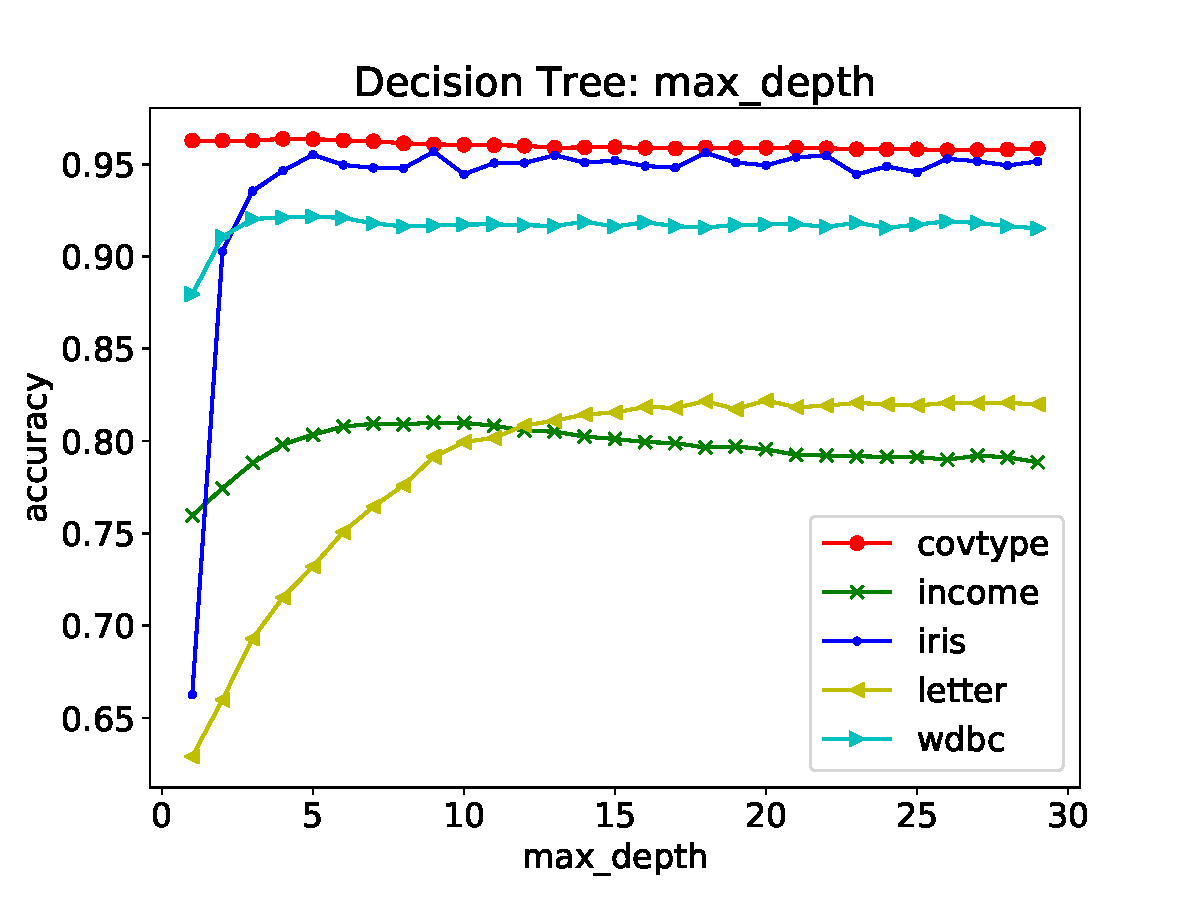
\includegraphics[width=\linewidth]{dt_hyperparam_max_depth}
						\caption{Decision Tree: \textit{max\_depth}}
						\label{fig:hyperparam_dt_max_depth}
					\end{subfigure}
					\begin{subfigure}[b]{.49\linewidth}
						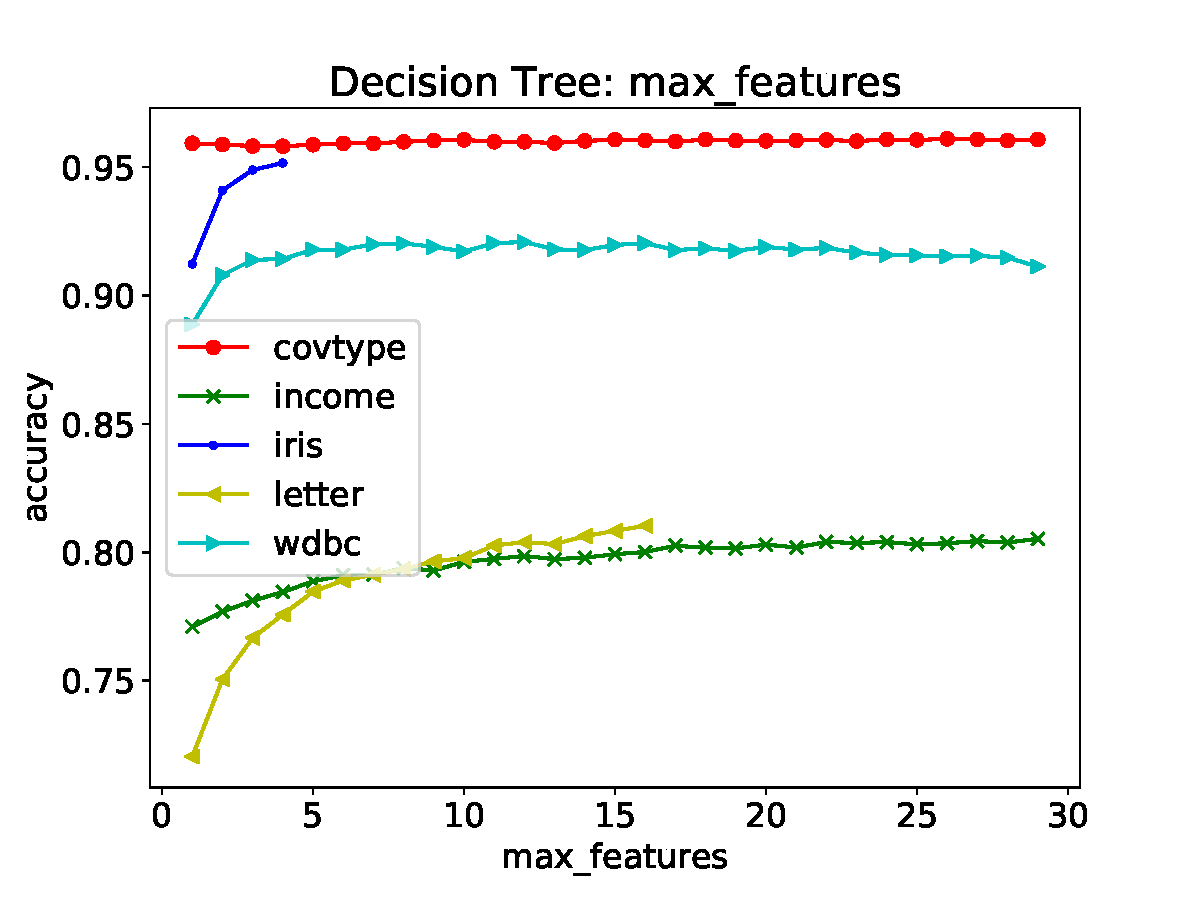
\includegraphics[width=\linewidth]{dt_hyperparam_max_features}
						\caption{Decision Tree: \textit{max\_features}}
						\label{fig:hyperparam_dt_max_features}
					\end{subfigure}
					
					\caption{Average cross-validated prediction accuracy by hyperparameter value for KNN (\ref{fig:hyperparam_knn_zoomed} and \ref{fig:hyperparam_knn_all}) and Decision Tree (\ref{fig:hyperparam_dt_max_depth} and \ref{fig:hyperparam_dt_max_features}), averaged over problems, shuffles, and train splits. (\ref{fig:hyperparam_knn_zoomed}) zooms in on a subset of the results shown in (\ref{fig:hyperparam_knn_all}) for greater detail. (\ref{fig:hyperparam_dt_max_depth}) depicts results for varying levels of \textit{max\_depth}, averaged over \textit{max\_features}, and vice versa in (\ref{fig:hyperparam_dt_max_features}).}
					\label{fig:hyperparam_knn_dt}
				\end{framed}
			\end{figure}
			
			% Hyperparam figures # 2
			\begin{figure}[h]
				\begin{framed}
					\centering
					
					\begin{subfigure}[b]{.49\linewidth}
						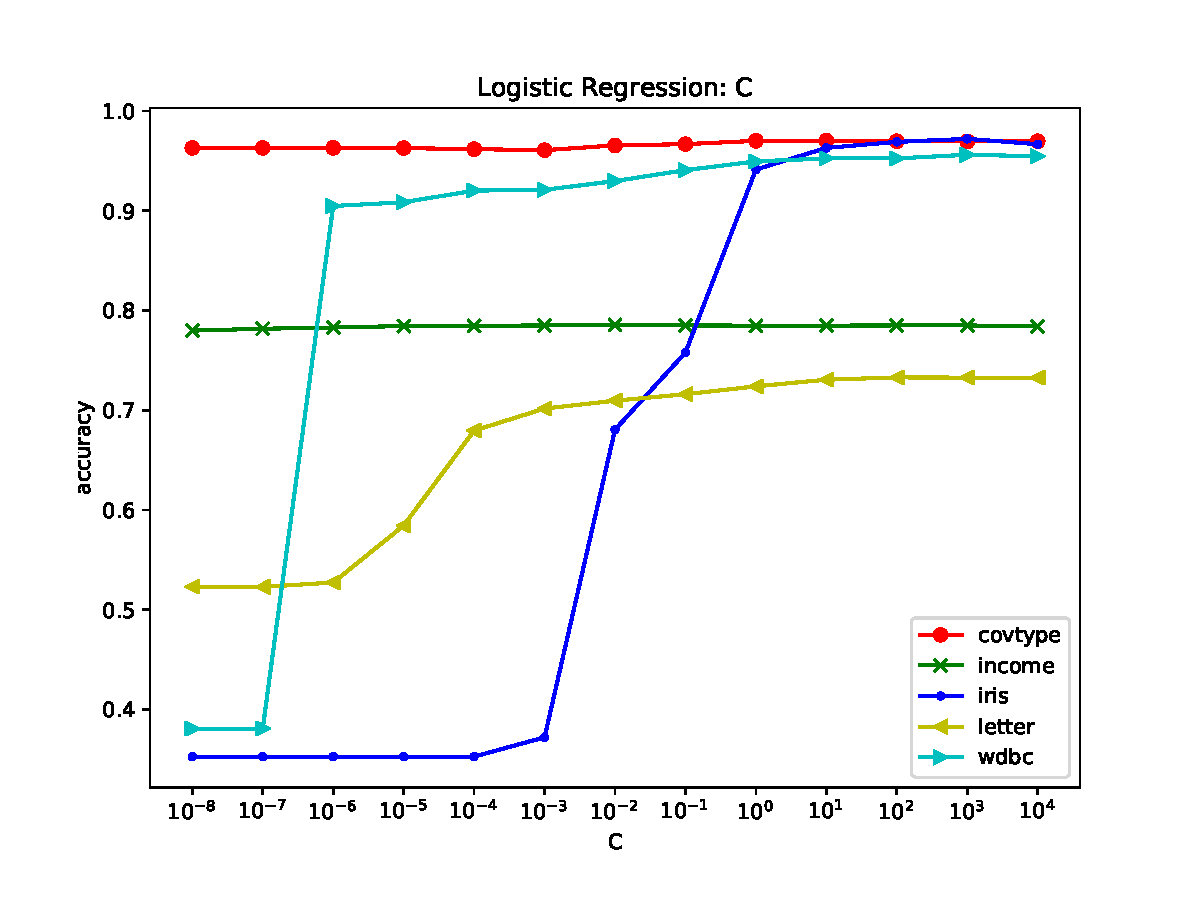
\includegraphics[width=\linewidth]{logreg_hyperparam}
						\caption{Logistic Regression: \textit{C}}
						\label{fig:hyperparam_logreg}
					\end{subfigure}
					\begin{subfigure}[b]{.49\linewidth}
						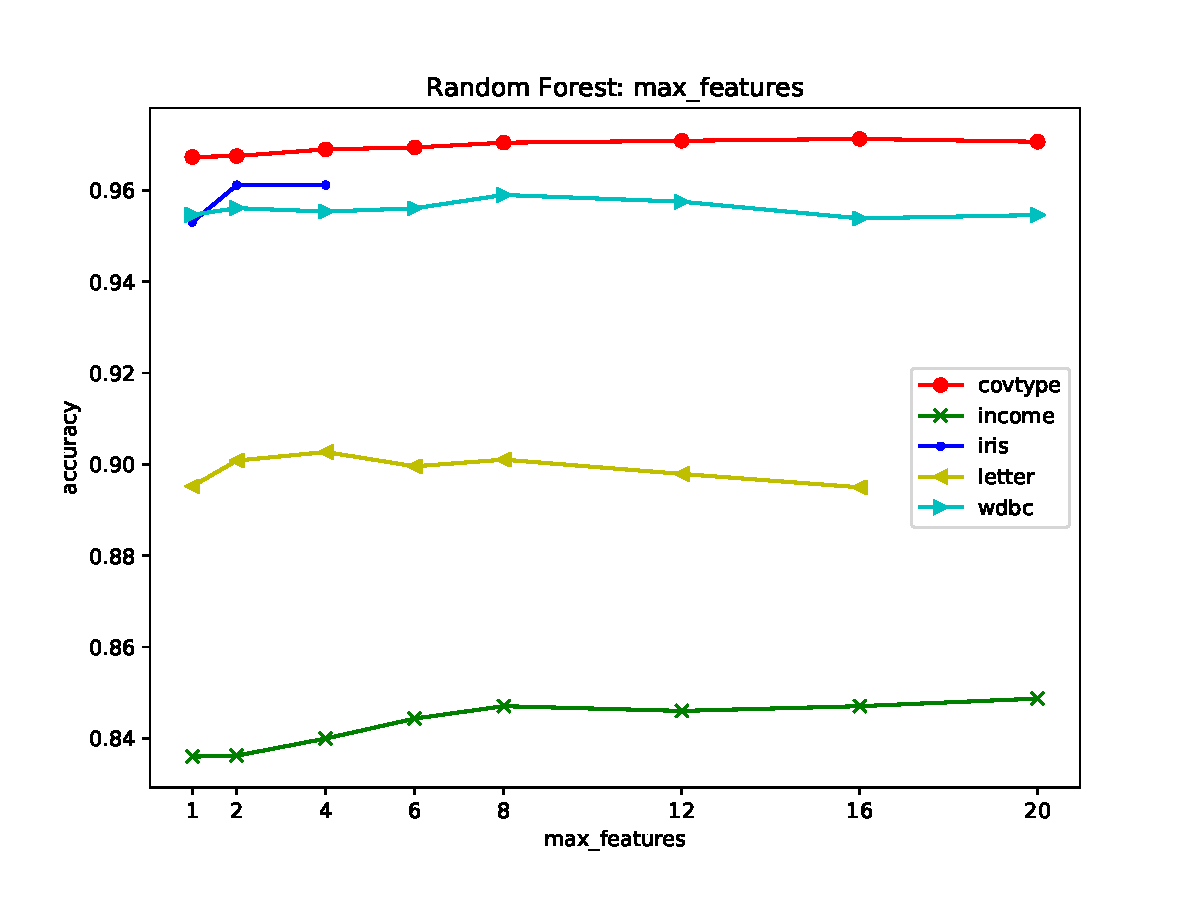
\includegraphics[width=\linewidth]{rf_hyperparam}
						\caption{Random Forest: \textit{n\_estimators}}
						\label{fig:hyperparam_rf}
					\end{subfigure}
					
					\begin{subfigure}[b]{.49\linewidth}
						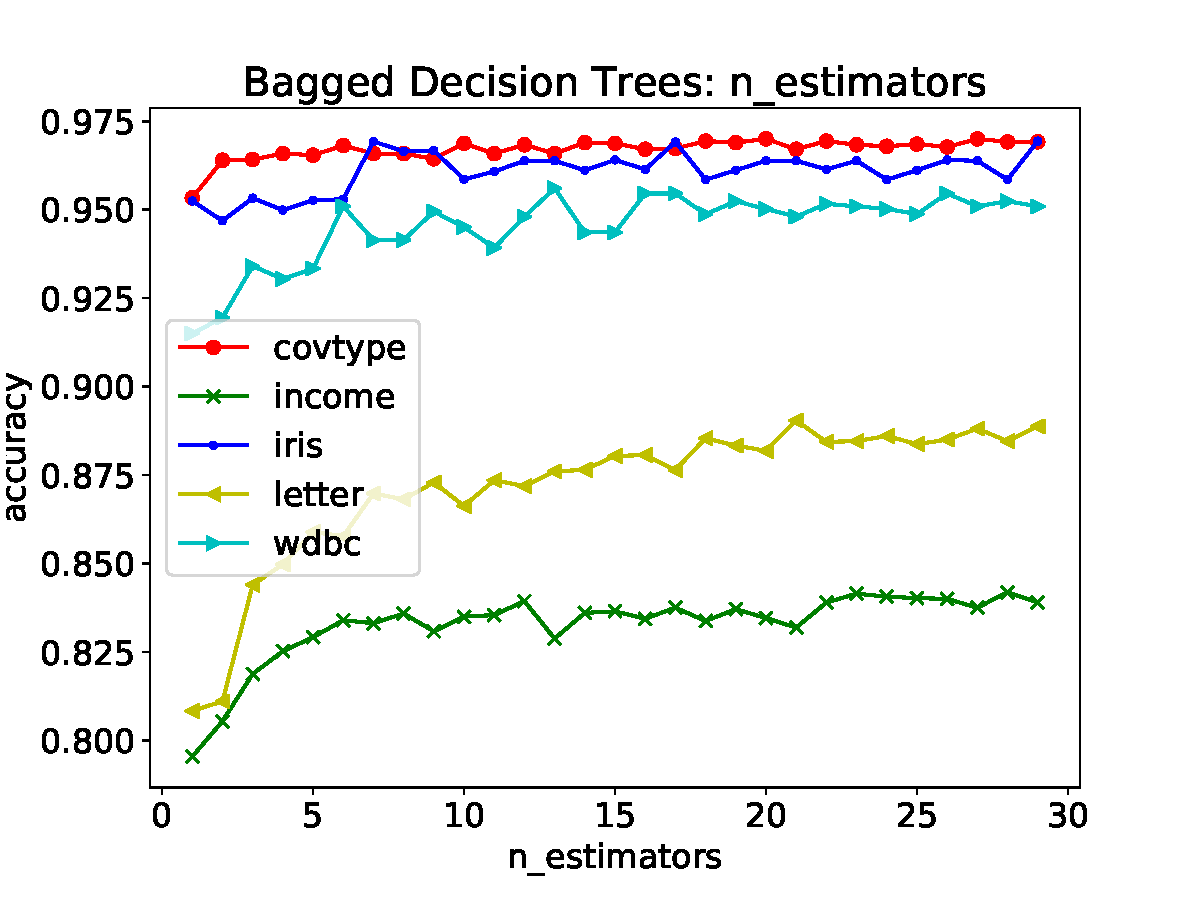
\includegraphics[width=\linewidth]{bagdt_hyperparam}
						\caption{Bagged Decision Trees: \textit{n\_estimators}}
						\label{fig:hyperparam_bagdt}
					\end{subfigure}
					\begin{subfigure}[b]{.49\linewidth}
						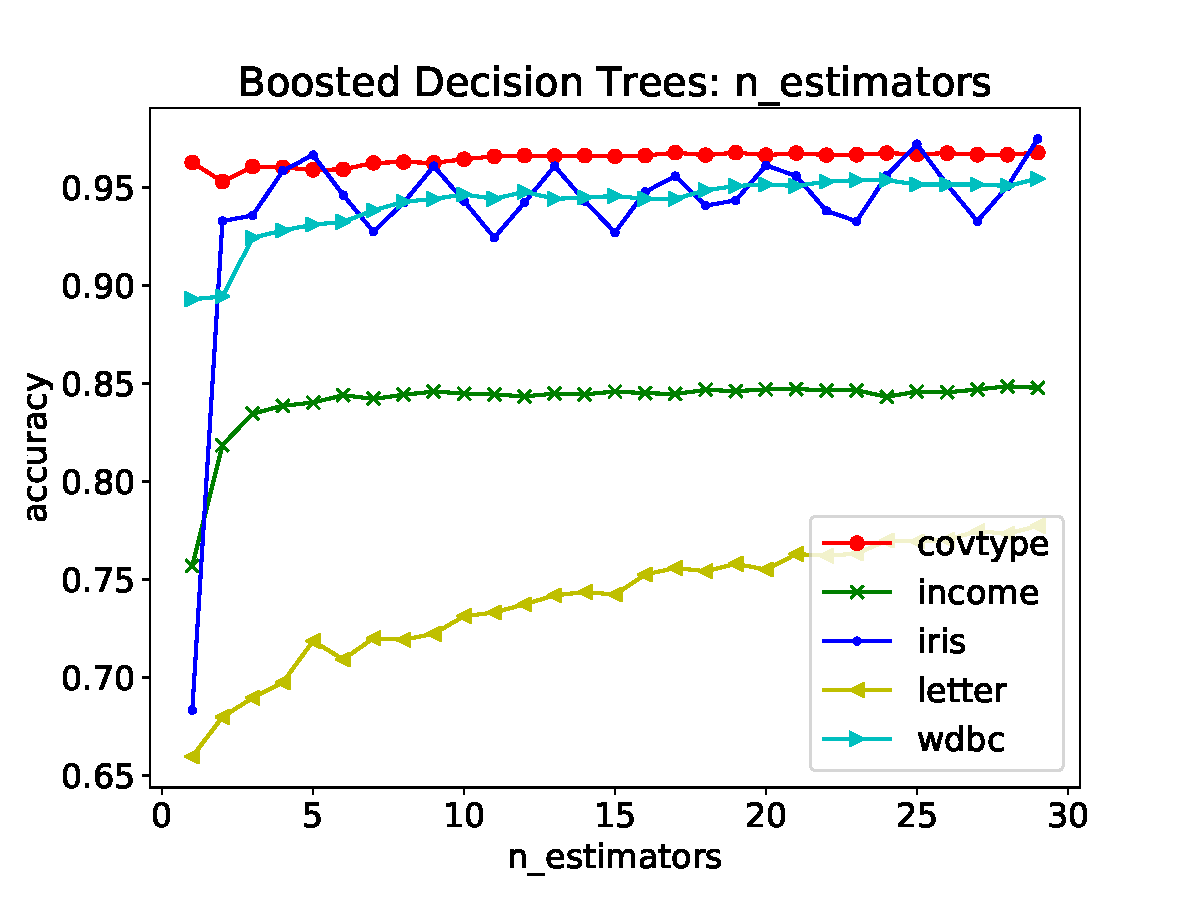
\includegraphics[width=\linewidth]{bstdt_hyperparam}
						\caption{Boosted Decision Trees: \textit{n\_estimators}}
						\label{fig:hyperparam_bstdt}
					\end{subfigure}
					
					\caption{Average cross-validated prediction accuracy by hyperparameter value for Logistic Regression (\ref{fig:hyperparam_logreg}), Random Forest (\ref{fig:hyperparam_rf}), Bagged Decision Trees (\ref{fig:hyperparam_bagdt}), and Boosted Decision Trees (\ref{fig:hyperparam_bstdt}).}
					\label{fig:hyperparam_others}
				\end{framed}
			\end{figure}
		
		\subsection{Train/Test split and Performance}
			The influence of the train split and the resulting relative sizes of training and testing sets on prediction accuracy is shown separately for training and testing accuracies in Figure \ref{fig:perf_by_trainsplit}.
			
			\begin{figure}[h]
				\begin{framed}
					\begin{subfigure}{.5\textwidth}
						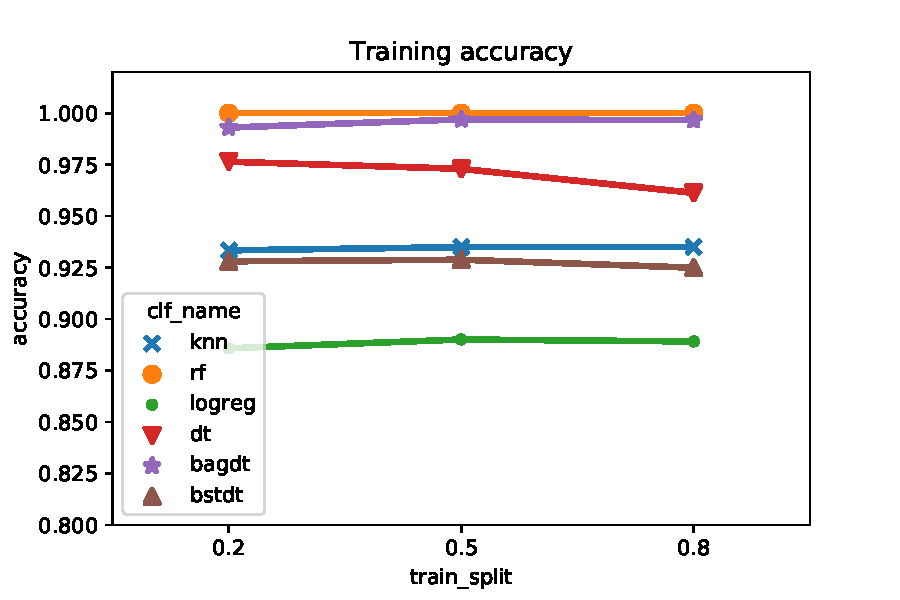
\includegraphics[width=\textwidth]{tr_acc_by_clf_trainsplit}
						\caption{Training accuracy}
						\label{fig:perf_by_trainsplit_tr}
					\end{subfigure}
					\begin{subfigure}{.5\textwidth}
						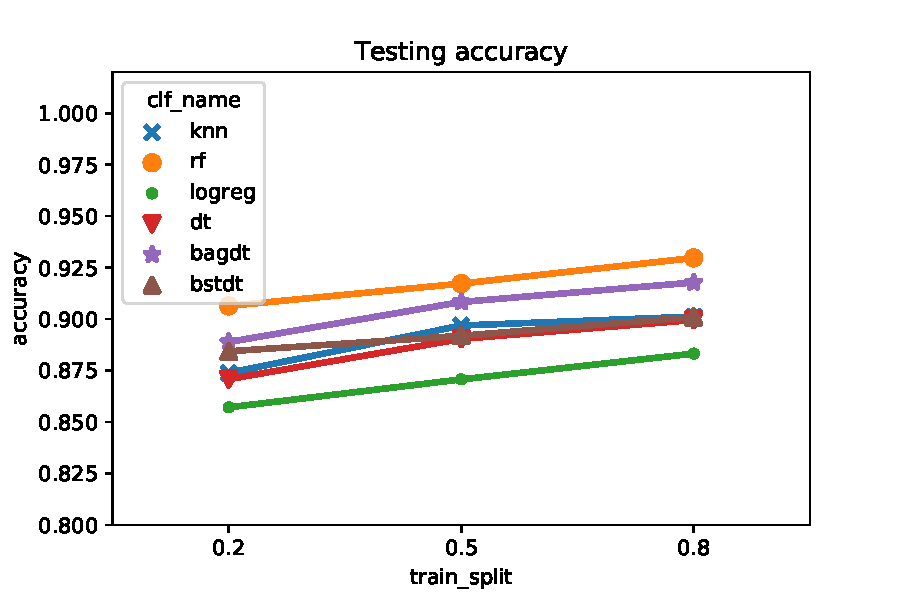
\includegraphics[width=\textwidth]{te_acc_by_clf_trainsplit}
						\caption{Testing accuracy}
						\label{fig:perf_by_trainsplit_te}
					\end{subfigure}
					\caption{Training (\ref{fig:perf_by_trainsplit_tr}) and testing (\ref{fig:perf_by_trainsplit_te}) accuracy by train split and classifier, averaged over problems and shuffles (rf: Random Forest, logreg: Logistic Regression, dt: Decision Tree, bagdt: Bagged Trees, bstdt: Boosted Trees)}
					\label{fig:perf_by_trainsplit}
				\end{framed}
			\end{figure}
		
		\subsection{Overall Classifier Performance}
			The estimates of overall classifier performance are based on the best hyperparameter combinations that were yielded by exhaustive grid search for each shuffle for \textit{train split} = .8. Table \ref{tab:best_hyperparams_by_problem_shuffles} lists these optimal hyperparameter values for each classifier, problem data set, and random shuffle. Based on models with these values, the prediction accuracy on the testing set was determined and averaged over the three shuffles. Table \ref{tab:test_acc_by_clf_and_problem} indicates the thus obtained average testing accuracies for each classifier by problem data set.
			
			Finally, testing accuracies were averaged over problems. The resulting overall mean testing performances and rank order is given by Table \ref{tab:clf_ranking}.
			
			% Model selection results: Best hyperparams
			\begin{table}[h]
				\caption{Best hyperparameter values after grid search by classifier and problem in each of three random shuffles (0.8 train split):}
				\label{tab:best_hyperparams_by_problem_shuffles}
				\resizebox{\textwidth}{!}{%
				\begin{tabular}{lllllll}
					\toprule
					& & \multicolumn{5}{c}{\textbf{Problem}} \\\cline{3-7}
					\rule{0pt}{3ex} \textbf{Classifier} & \textbf{Hyperparam.} &         \textbf{COVTYPE} &           \textbf{INCOME} &               \textbf{IRIS} &              \textbf{LETTER} &                 \textbf{WDBC} \\
					\midrule
					bagdt & \textit{n\_estimators} &         3,27,14 &         26,25,28 &             9,29,7 &            21,14,18 &              13,9,16 \\
					bstdt & \textit{n\_estimators}  &        24,19,12 &         28,18,18 &            5,29,24 &            29,28,24 &             21,29,10 \\
					\multirow{2}{*}{dt} & \textit{max\_depth} &           3,5,4 &            8,4,6 &              9,9,3 &            18,19,18 &                6,5,6 \\
					& \textit{max\_features} &        18,24,19 &         18,24,26 &              3,4,4 &             10,15,6 &              7,11,15 \\
					knn & \textit{n\_neighbors} &           4,5,9 &           8,6,17 &             12,9,1 &               1,1,1 &                9,7,7 \\
					logreg & \textit{C} &  $10^2$,1,10 &  $10^{-5}$,01,01 &  10,$10^3$,$10^2$ &  $10^2$,$10^3$,$10^2$ &  $10^3$0,10,$10^3$ \\
					rf & \textit{max\_features} &        20,16,16 &          20,16,8 &              1,2,2 &               4,2,8 &               12,8,8 \\
					\bottomrule
				\end{tabular}}
			
			\end{table}
			
			% Overall average results of clfs on datasets
			\begin{table}[h]
				\captionbox{Classifier testing accuracy by problem, averaged over shuffles (0.8 train split):\label{tab:test_acc_by_clf_and_problem}}{
				\begin{tabular}{lrrrrr}
					\toprule
					\textbf{Classifier} & \textbf{WDBC} & \textbf{INCOME} & \textbf{IRIS} & \textbf{COVTYPE} & \textbf{LETTER} \\
					\midrule
					Bagged Trees  & .968 &   .833 & .944 &    .971 &   .873 \\
					Boosted Trees  & .968 &   .840 & .956 &    .971 &   .771 \\
					Decision Tree     & .953 &   .799 & .956 &    .970 &   .820 \\
					KNN    & .950 &   .757 & .933 &    .967 &   \textbf{.899} \\
					Logistic Regression & .968 &   .792 & \textbf{.967} &    .968 &   .721 \\
					Random Forest     & \textbf{.982} &   \textbf{.848} & .944 &    \textbf{.976} &   .897 \\
					\bottomrule
				\end{tabular}}
			\end{table}
			
			% Overall average results of clfs, sorted
			\begin{table}[h]
				\centering
				\caption{Overall average testing accuracy by classifier and comparison with results from \cite{caruana_empirical_2006}}\label{tab:clf_ranking}
				\begin{subtable}[t]{2.9in}
					\centering
					\caption{Ranked classifiers by testing accuracy, averaged over problems and shuffles (0.8 train split):}\label{table:1b}
					\begin{tabular}{llr}
						\toprule
						\textbf{Rank} & {\textbf{Classifier}} & \textbf{Accuracy} \\
						\midrule
						1 & Random Forest     &     .930 \\
						2 & Bagged Trees  &     .918 \\
						3 & KNN    &     .901 \\
						4 & Boosted Trees  &     .901 \\
						5 & Decision Tree     &     .900 \\
						6 & Logistic Regression &     .883 \\
						\bottomrule
					\end{tabular}
				\end{subtable}
				\quad
				\begin{subtable}[t]{2.9in}
					\centering
					\caption{Results from \cite{caruana_empirical_2006}}
					\begin{tabular}{llr}
						\toprule
						\textbf{Rank} & {\textbf{Classifier}} & \textbf{Accuracy} \\
						\midrule
						1 & Random Forest     &     .872 \\
						2 & Bagged Trees  &     .846 \\
						3 & Boosted Trees  &     .834 \\
						3 & KNN    &     .756 \\
						5 & Decision Tree     &     .647 \\
						6 & Logistic Regression &     .636 \\
						\bottomrule
					\end{tabular}
				\end{subtable}
			\end{table}
	
	\section{Conclusion}
		The present analysis managed to replicate a subset of the empirical results from \cite{caruana_empirical_2006}. The higher testing accuracies achieved in this study (see Table \ref{tab:clf_ranking}) indicate that the problems were on average easier. However, the ranking orders are identical except for third and fourth ranked classifiers KNN and Boosted Trees, which occur in reversed order in this ranking (but their scores were very close to each other).
		
		Regarding the results of different train-test-splits (see Figure \ref{fig:perf_by_trainsplit}), the expected result of higher testing accuracies with larger relative training set sizes could also be replicated.
		
		Considering the relationship between hyperparameter and prediction accuracy, the classifiers studied here can be divided into three groups:
		
		\noindent\textbf{Type 1: Monotonic relationship between hyperparameter and performance}\\
		For \textit{max\_features} in Decision Trees, testing performance stagnates for values higher than approximately 8 for all problems other than INCOME and LETTER, where testing accuracy kept slowly increasing after that value. The regularization parameter $C$ in Logistic Regression showed an interesting influence on testing accuracy, which forms the shape of a sigmoid in the case of the IRIS, LETTER, and WDBC problems. In both Bagged and Boosted Decision Trees, higher values of \textit{n\_estimators} correspond to higher testing accuracies.
		
		\noindent\textbf{Type 2: Local optimum or quick convergence}
		In Decision Trees, testing accuracy converged quickly towards an upper limit with increasing values of \textit{max\_depth}, except for the problem INCOME, where testing accuracy started to slowly decrease after a hyperparameter value of approximately 10. The number $K$ of nearest neighbors considered in KNN seemed to have a ``sweet spot'' in form of a local maximum in testing accuracy in the lower range of values, but after an initial steep increase for most problems. A notable exception is the LETTER data set, where lower values of $K$ are better (see also Table \ref{tab:best_hyperparams_by_problem_shuffles}).
		
		\noindent\textbf{Type 3: Unclear}
		The relationship between $n\_estimators$ and testing accuracy in Random Forest is less clear. For WDBC, there is a slight positive correlation, whereas for LETTER, it is slightly negative. These results might be due to a ceiling effect, since Random Forest achieved very high overall.
		
		These results seem to imply systematic relationships between hyperparameters and testing accuracy. This makes the further development of Machine Learning algorithms that aim at automatically tuning model hyperparameters even more promising. The present study also visualized how much these relationships differ between different data sets, which shows that optimal hyperparameters indeed seem to be a problem that needs to be learned from data.
	
	\section{Bonus Points}
		The code that this analysis is based on is highly generalized and abstracts over algorithms, data, train splits, and random shuffles. Each of these can conveniently be adjusted in the configuration part of the script, and calling one function is then enough to run all loops required for the present study (siehe code below). New classifiers can be implemented by adding a link to a scikit-learn estimator interface compatible class in \textit{CLF\_DICT}. The grid of hyperparameters to be varied is set by entries in \textit{CLF\_PARAM\_DICT}, using their scikit-learn estimator interface argument names. Similarly, new data sets can be added by adding named (X, y) tuples to \textit{DATA\_DICT}. Any number of train split sizes can be indicated in \textit{TRAIN\_SPLITS}, and the maximal data size to be computed is determined by \textit{MAX\_DATA\_SIZE}. The number of randomly drawn sub-samples from the data set is set by \textit{N\_SHUFFLES}. \textit{CV} is the number of cross-validation folds, and \textit{KNN\_FILLUP} is the number of evenly spaced values of $K$ for KNN that are added to the parameter grid between the highest number indicated in CLF\_PARAM\_DICT and the maximum valid number determined by $\frac{|DATASET|}{CV}$ for each dataset. Listing \ref{listing:code} shows the code that is used for this analysis. All settings and loops are set using the uppercase configuration constants, and a call of \mint{python}{BigLoop.run()} runs the whole analysis with all required loops.
		
		\begin{listing}
		\begin{minted}{python}

CLF_DICT       = {'logreg': linear_model.LogisticRegression(),
                  'knn':    neighbors.KNeighborsClassifier(),
                  'rf':     ensemble.RandomForestClassifier(),
                  'svm':    svm.SVC(),
                  'dt':     tree.DecisionTreeClassifier(),
                  'bagdt':  ensemble.BaggingClassifier(),
                  'bstdt':  ensemble.AdaBoostClassifier()}
                  
CLF_PARAM_DICT = {'knn':    {'n_neighbors':  np.arange(1, 31)},
                  'rf':     {'n_estimators': np.array([1024]),
                  'max_features': np.array([1, 2, 4, 6, 8, 12, 16, 20])},
                  'logreg': {'C': np.array([1e-8, 1e-7, 1e-6, 1e-5, 1e-4,
                  1e-3, 1e-2, 1e-1, 1e0, 1e1, 1e2, 1e3, 1e4])},
                  'dt':     {'max_depth':    np.arange(1, 30),
                  'max_features': np.arange(1, 30)},
                  'bagdt':  {'n_estimators': np.arange(1, 30)},
                  'bstdt':  {'n_estimators': np.arange(1, 30)}}

DATA_DICT       = {'wdbc':      (wdbc_X, wdbc_y),
                  'income':    (income_X, income_y),
                  'iris':      (iris_X, iris_y),
                  'covtype':   (covtype_X, covtype_y),
                  'letter':    (letter_X, letter_y)}

MAX_DATA_SIZE  = 2000
TRAIN_SPLITS   = [0.2, 0.5, 0.8]
N_SHUFFLES     = 3
CV             = 5
KNN_FILLUP     = 10

loop = BigLoop(DATA_DICT, CLF_PARAM_DICT, TRAIN_SPLITS, N_SHUFFLES, CV,
knn_fillup=KNN_FILLUP, method='grid_search', n_jobs=4)
loop.run()
		\end{minted}
		\caption{Code used for this analysis, using the class \textit{BigLoop}}
		\label{listing:code}
		\end{listing}
	
		The BigLoop class already has a method included that allows to plot testing accuracy by hyperparameter for a given classifier and hyperparameter, averaging over shuffles and train splits. Another big advantage of this implementation is that the complete analysis, including the data, parameter combinations, results, and involved sklearn objects can be saved to one Pickle file, which can then quickly be loaded for further analysis without having to re-run the whole analysis.
		
		The code that this analysis is based on is completely available on GitHub (\url{https://github.com/phi1eas/118a_project}), including the scripts that generated all plots and the \LaTeX \hspace{.2em} code underlying the tables in this report from experiment results saved in a bigloop.pkl file.
		
		\vskip 0.2in
		\bibliography{118a}
	
	
	
	
	
	
%	\newpage
%	
%	\appendix
%	\section*{Appendix A.}
%	\label{app:theorem}
	
	
	
	
\end{document}